\section{Đánh giá định lượng và định tính trên tập kiểm thử độc lập}
\label{sec:danh_gia_test_phan_tang}

\subsection{Đánh giá so sánh định lượng trên tập kiểm thử độc lập}

Sau khi đóng băng cấu hình được chọn trên tập Validation, đánh giá được thực hiện trên tập kiểm thử độc lập gồm \textbf{839 ảnh Sentinel-1A} (chứa tổng cộng $3\,182$ đối tượng dầu Ground Truth) và tập kiểm thử ngoài cảm biến gồm \textbf{776 ảnh ALOS PALSAR} (chứa $3\,994$ đối tượng dầu Ground Truth).

Bảng~\ref{tab:model_comparison} trình bày chi tiết kết quả định lượng tổng hợp, gồm cả cách tính Micro-averaging và Macro-averaging ($\text{mean} \pm \text{SD}$ giữa các ảnh).

\begin{table}[!htbp]
\centering
\caption{Đánh giá so sánh hiệu năng trên tập kiểm thử độc lập (839 ảnh Sentinel-1A và 776 ảnh ALOS PALSAR) theo giao thức ghép cặp Hungarian ở ngưỡng $\IoU \ge 0.5$.}
\label{tab:model_comparison}
\begingroup
\setlength{\tabcolsep}{2pt}
\renewcommand{\arraystretch}{1.2}
\resizebox{\textwidth}{!}{%
\begin{tabular}{|>{\raggedright\arraybackslash}p{3.2cm}|c|*{9}{>{\centering\arraybackslash}p{1.82cm}|}}
\hline
\textbf{Phương pháp} & \textbf{Ảnh} & \textbf{TP} & \textbf{FP} & \textbf{FN} & \textbf{Prec} & \textbf{Rec} & \textbf{Obj F1} & \textbf{Pix IoU} & \textbf{FP/ảnh} & \begin{tabular}{@{}c@{}}\textbf{Edge / Int}\\\textbf{Recall}\end{tabular} \\ \hline
\textit{Baseline (Ảnh thô + Otsu, $A_{\min} = 16$)} & 839 & 426 & $49\,182$ & $2\,756$ & 0.0086 & 0.1339 & 0.0161 & 0.4367 & 58.62 & 0.1979 / 0.0038 \\ \hline
\textit{Lee 7$\times$7 + Otsu ($A_{\min} = 64$, Không Clf)} & 839 & $1\,018$ & $12\,495$ & $2\,164$ & 0.0753 & \textbf{0.3199} & 0.1220 & 0.5867 & 14.89 & \textbf{0.4221} / \textbf{0.1124} \\ \hline
\textbf{Pipeline + LinearSVM ($A_{\min} = 64$, Đề xuất)} & 839 & 996 & $\mathbf{2\,923}$ & $2\,186$ & \textbf{0.2541} & 0.3130 & \textbf{0.2805} & \textbf{0.6614} & \textbf{3.48} & 0.4156 / 0.1048 \\ \hline
\quad \textit{Macro từng ảnh ($\text{mean} \pm \text{SD}$)$^{\dagger}$} & \multicolumn{4}{c|}{--} & $0.356 \pm 0.336$ & $0.446 \pm 0.382$ & $0.349 \pm 0.317$ & $0.577 \pm 0.261$ & $3.48 \pm 3.97$ & -- \\ \hline
\textit{Ngoài cảm biến: PALSAR (LinearSVM, $A_{\min} = 64$)} & 776 & $1\,441$ & $2\,305$ & $2\,553$ & 0.3847 & 0.3608 & 0.3724 & 0.6423 & 2.97 & 0.4587 / 0.1890 \\ \hline
\quad \textit{Macro từng ảnh ($\text{mean} \pm \text{SD}$)$^{\ddagger}$} & \multicolumn{4}{c|}{--} & $0.465 \pm 0.342$ & $0.438 \pm 0.338$ & $0.412 \pm 0.312$ & $0.579 \pm 0.234$ & $2.97 \pm 3.43$ & -- \\ \hline
\end{tabular}%
}
\par\vspace{3pt}
{\raggedright\footnotesize
$^{\dagger}$Cỡ mẫu xác định trên Sentinel-1A (839 ảnh): $n_{\text{Prec}}=786$, $n_{\text{Rec}}=808$, $n_{\text{F1}}=n_{\text{IoU}}=814$ (25 ảnh $R_0$ có $\text{TP}=\text{FP}=\text{FN}=0$).\par
$^{\ddagger}$Cỡ mẫu xác định trên ALOS PALSAR (776 ảnh): $n_{\text{Prec}}=705$, $n_{\text{Rec}}=731$, $n_{\text{F1}}=n_{\text{IoU}}=734$ (42 ảnh $R_0$ có $\text{TP}=\text{FP}=\text{FN}=0$).\par}
\endgroup
\end{table}

\begin{figure}[!htbp]
\centering
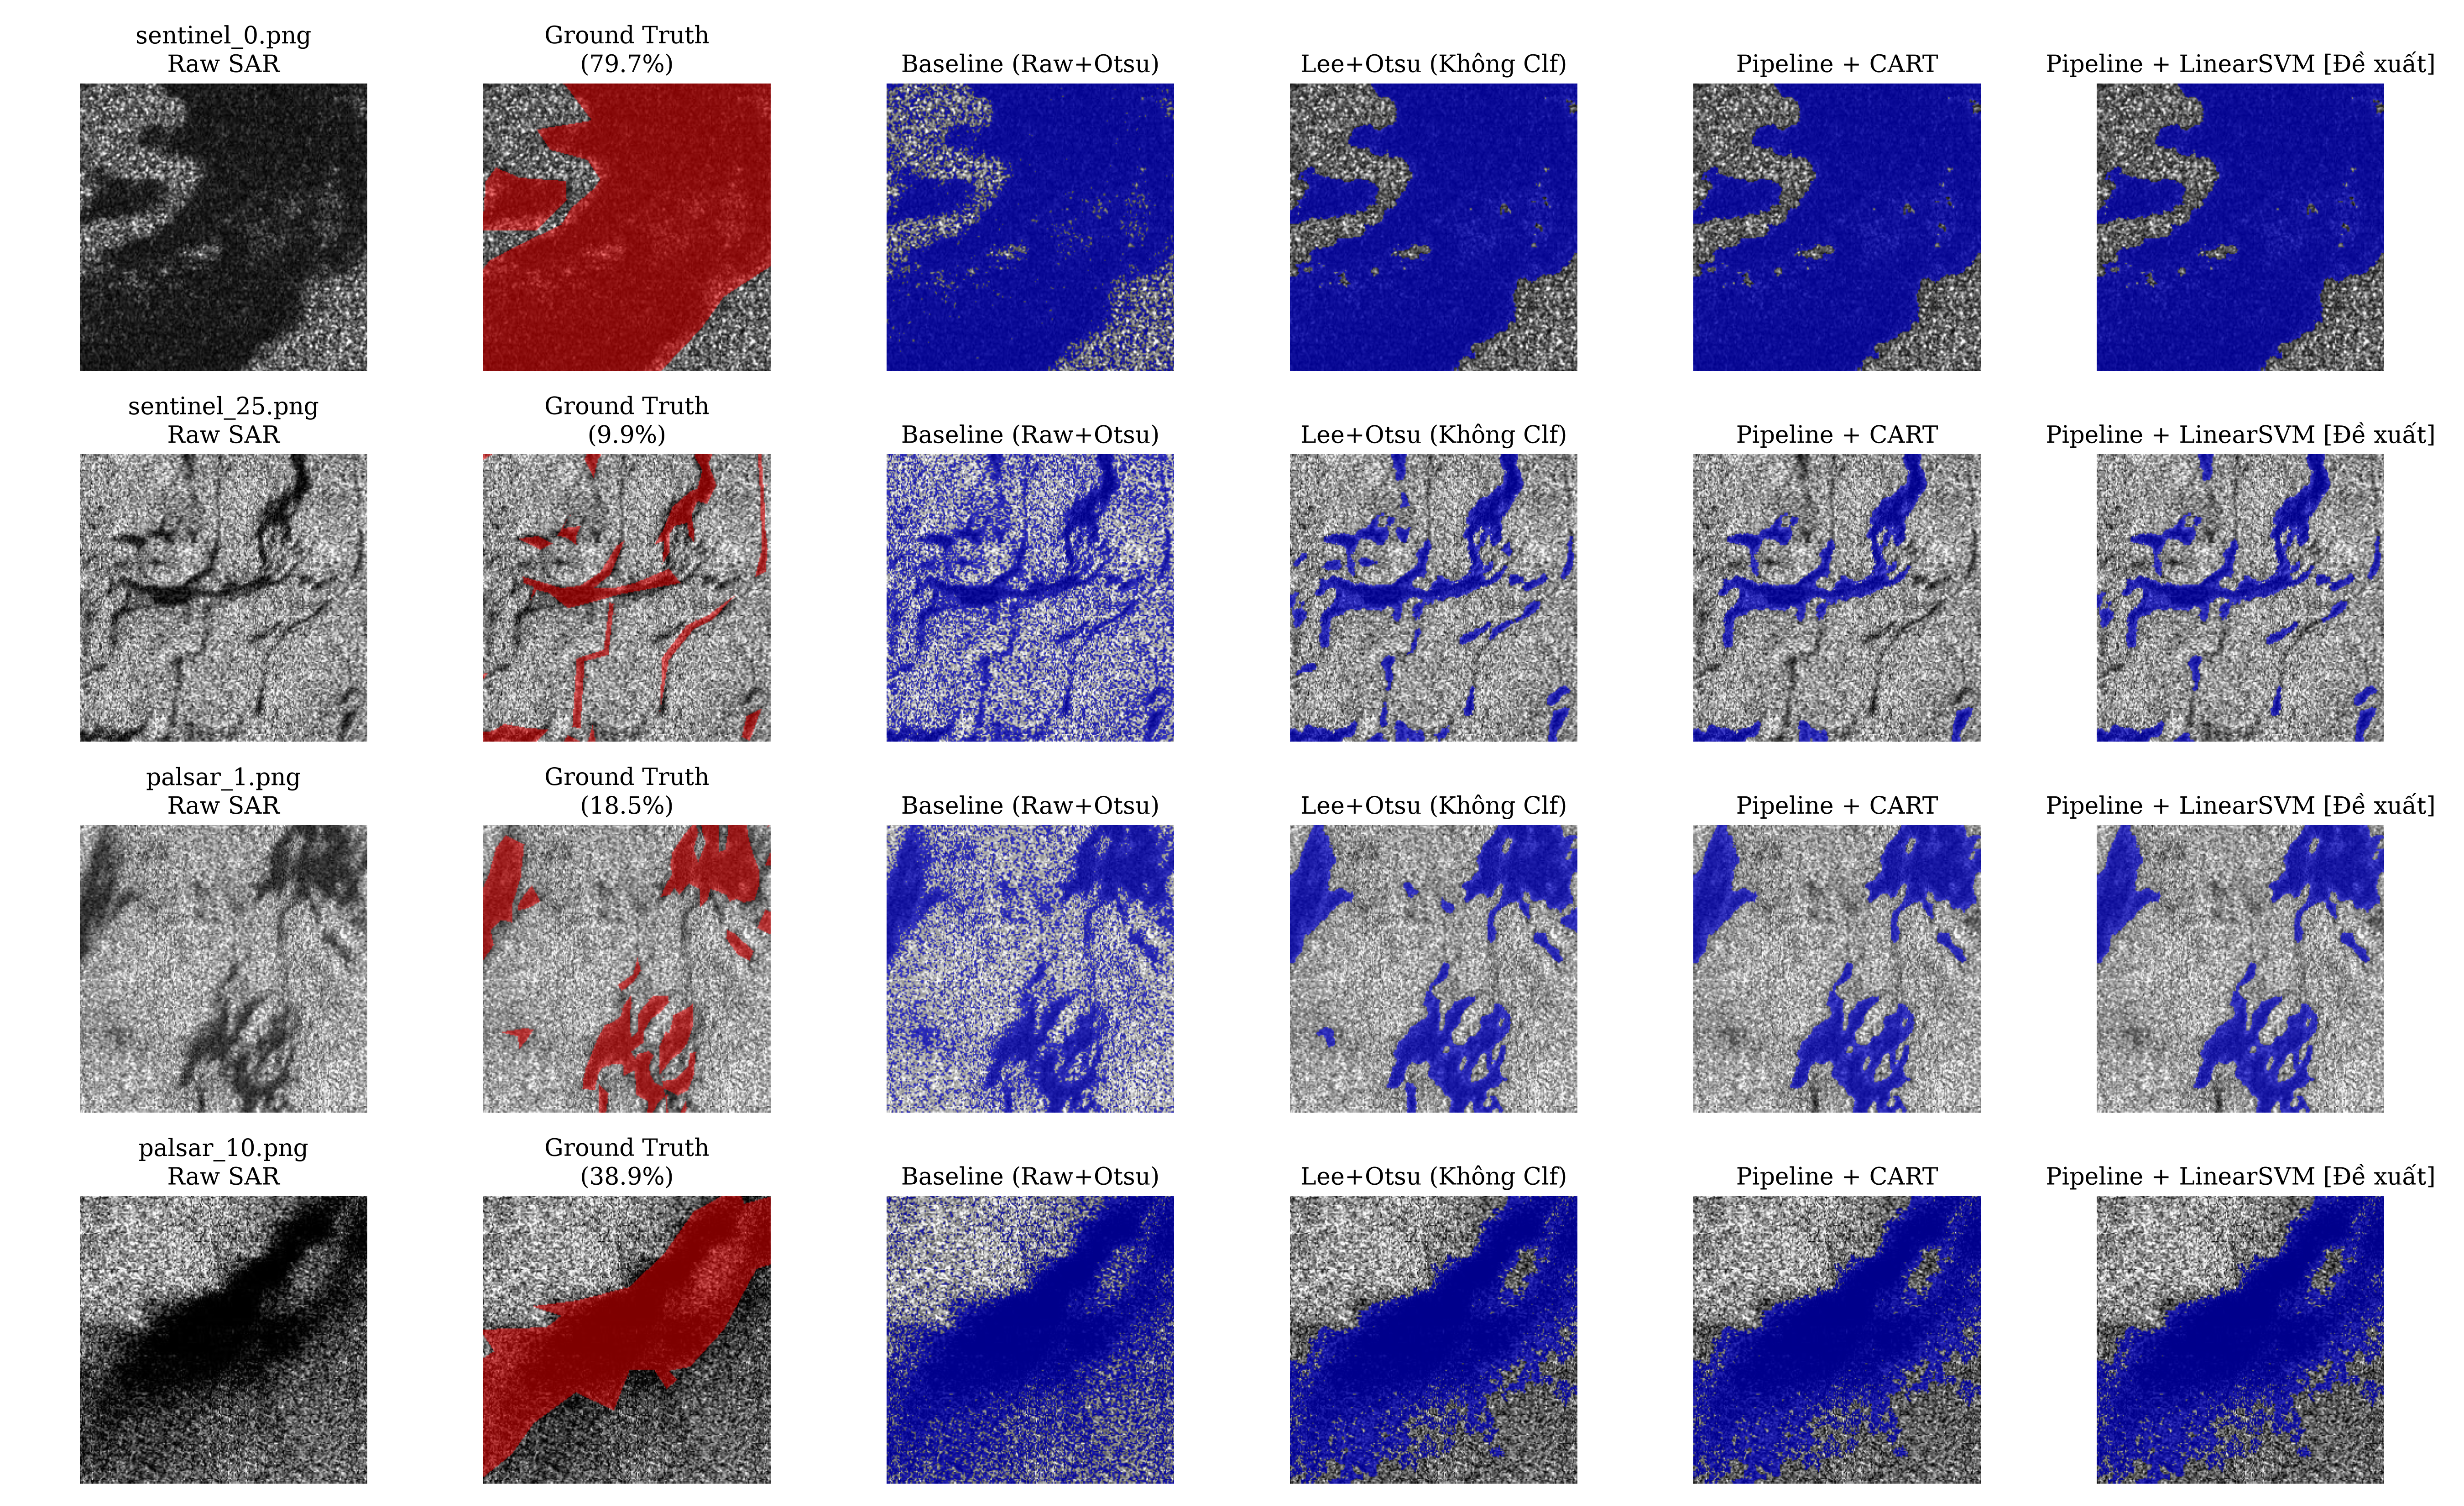
\includegraphics[width=\textwidth]{figures/fig7_qualitative_comparison.png}
\caption{Đối sánh định tính kết quả phân đoạn giữa các phương pháp trên 4 cảnh SAR viễn thám đại diện: Cột 1: Ảnh gốc; Cột 2: Mặt nạ Ground Truth; Cột 3: Baseline thô; Cột 4: Lọc Lee + Otsu (Không classifier); Cột 5: Pipeline + CART; Cột 6: Pipeline + LinearSVM (Đề xuất).}
\label{fig:qualitative_comparison}
\end{figure}

Hình~\ref{fig:qualitative_comparison} minh họa đối sánh định tính trên 4 cảnh SAR điển hình. Kết quả định lượng cho thấy:
\begin{enumerate}
    \item \textbf{Cắt giảm $76.6\%$ số vùng báo nhầm:} So với cấu hình tạo ứng viên không dùng classifier ($\text{TP}=1\,018, \text{FP}=12\,495$), việc tích hợp bộ phân loại LinearSVM đã loại bỏ $9\,572$ vùng tối giả, đưa tỷ lệ cảnh báo sai từ $14.89$ xuống còn $3.48$ FP/ảnh.
    \item \textbf{Bảo toàn $97.8\%$ số đối tượng đúng:} LinearSVM giữ lại $996 / 1\,018$ TP của giai đoạn ứng viên (chỉ giảm 22 đối tượng), nâng Precision lên $3.37$ lần (từ $0.0753$ lên $0.2541$), nâng Object F1 từ $0.1220$ lên $0.2805$ ($\Delta\text{F1} = +0.1586$, 95\% CI $[+0.1474, +0.1706]$) và Pixel IoU đạt $0.6614$.
\end{enumerate}

\subsection{Hiệu năng phân tầng theo 5 chế độ diện tích và khả năng chuyển giao ngoài cảm biến}

Bảng~\ref{tab:regime_breakdown} và Hình~\ref{fig:regime_sensor} phân tích chi tiết hiệu năng của hệ thống theo từng lát cắt dữ liệu vật lý ($R_0 \to R_4$) trên cả hai cảm biến Sentinel-1A và ALOS PALSAR.

\begin{figure}[!htbp]
\centering
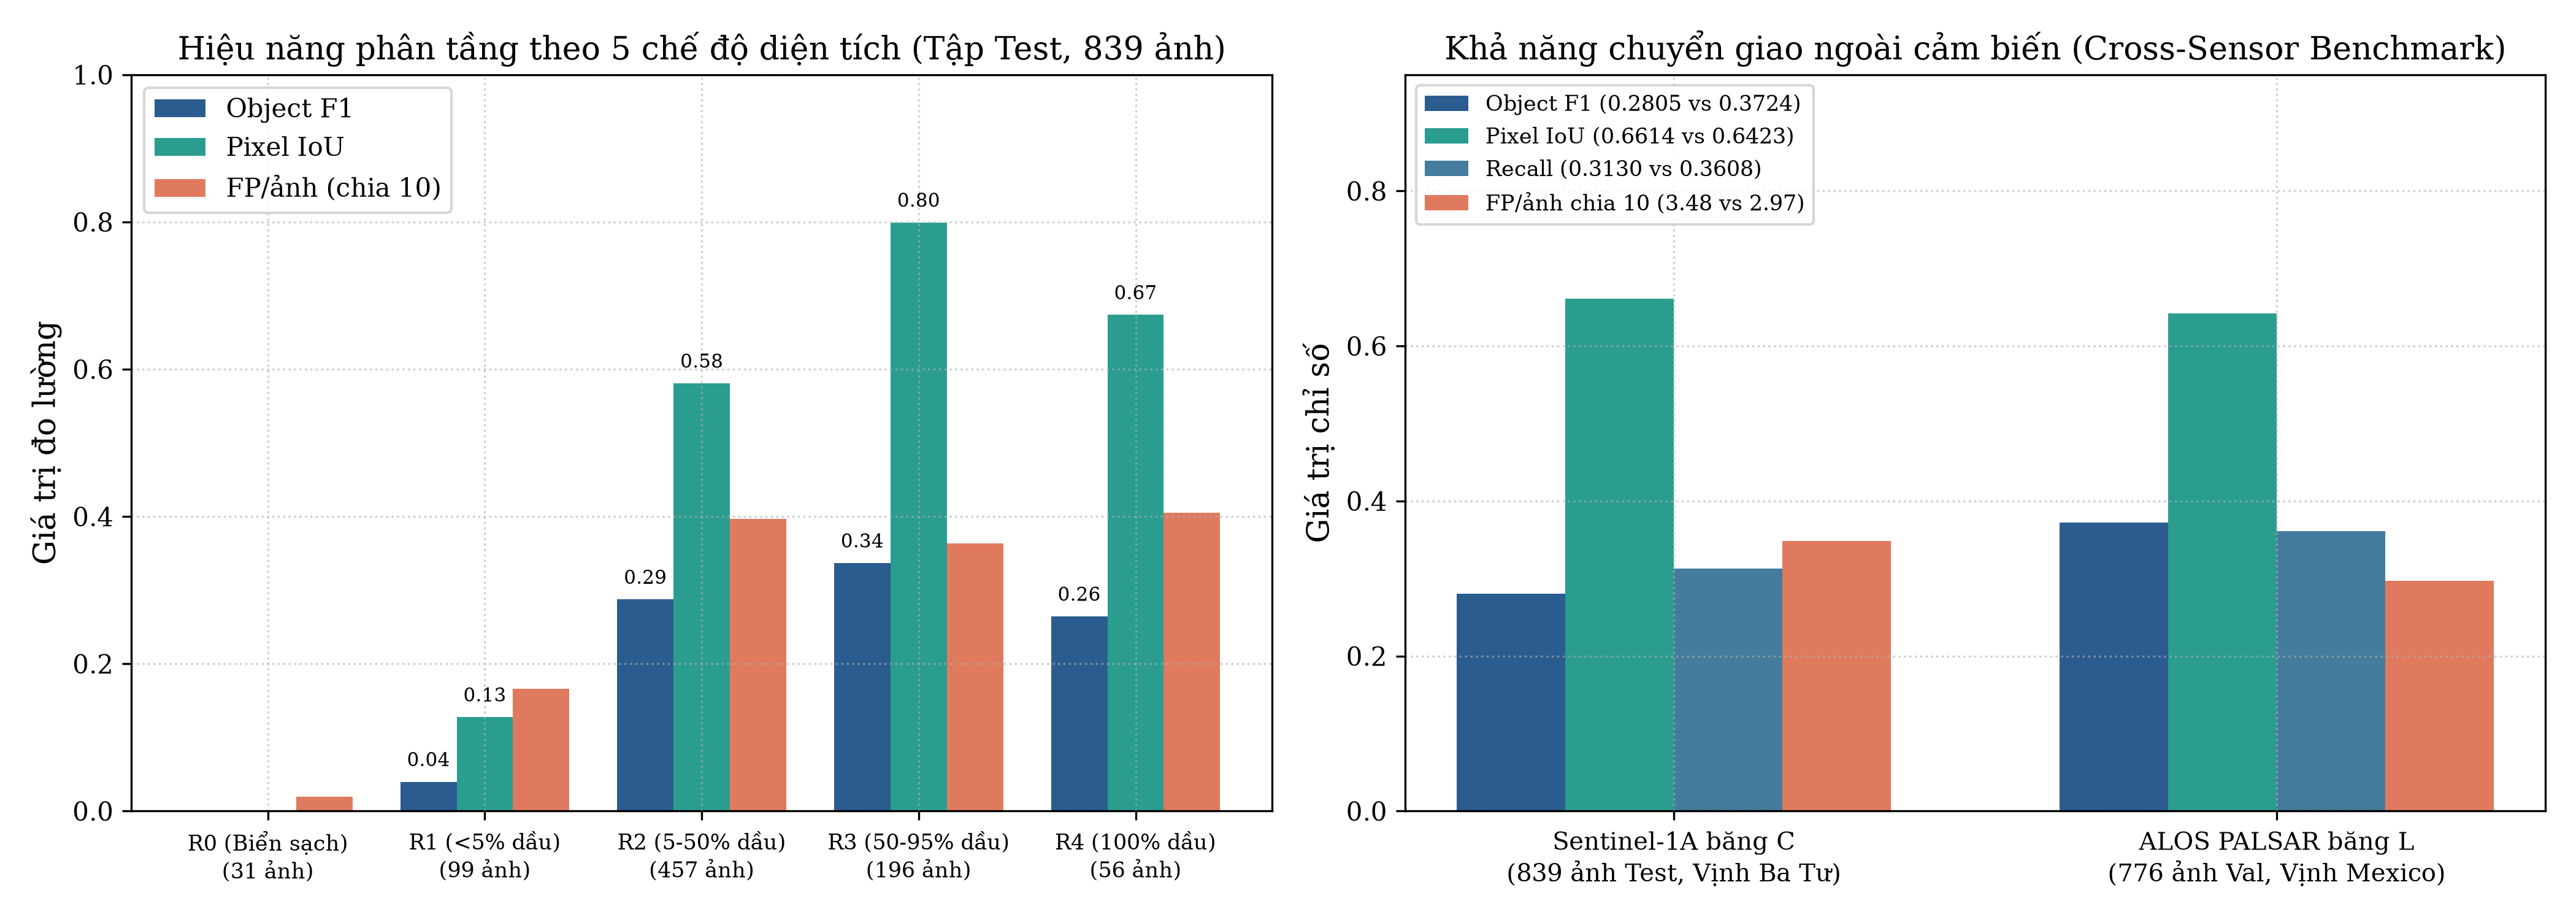
\includegraphics[width=0.96\textwidth]{figures/fig8_regime_sensor_performance.png}
\caption{Hiệu năng phân tầng theo 5 chế độ diện tích dầu ($R_0 \to R_4$) trên 839 ảnh Test Sentinel-1A (trái) và chuyển giao sang 776 ảnh ALOS PALSAR (phải).}
\label{fig:regime_sensor}
\end{figure}

\begin{table}[!htbp]
\centering
\small
\caption{Chi tiết hiệu năng phân tầng theo 5 chế độ diện tích dầu ($R_0 \to R_4$) trên hai tập kiểm thử độc lập.}
\label{tab:regime_breakdown}
\resizebox{\textwidth}{!}{%
\begin{tabular}{|l|c|c|c|c|c|c|c|}
\hline
\textbf{Chế độ diện tích} & \textbf{Số ảnh} & \textbf{TP} & \textbf{FP} & \textbf{FN} & \textbf{Object F1} & \textbf{Pixel IoU} & \textbf{FP / ảnh} \\ \hline
\multicolumn{8}{|l|}{\textit{Tập kiểm thử Sentinel-1A (839 ảnh, Vịnh Ba Tư, băng C, VV):}} \\ \hline
$R_0$ (Biển sạch, 0\% dầu) & 31 & 0 & 6 & 0 & N/A & N/A & \textbf{0.19} \\ \hline
$R_1$ (Vết dầu nhỏ, $<5\%$) & 99 & 9 & 164 & 271 & 0.0397 & 0.1276 & 1.66 \\ \hline
$R_2$ (Dải dầu trung bình, $5\text{--}50\%$) & 457 & 693 & $1\,814$ & $1\,624$ & 0.2873 & 0.5808 & 3.97 \\ \hline
$R_3$ (Dầu diện rộng, $50\text{--}95\%$) & 196 & 250 & 712 & 273 & \textbf{0.3367} & \textbf{0.7993} & 3.63 \\ \hline
$R_4$ (Ngập dầu toàn phần, $\ge 95\%$) & 56 & 44 & 227 & 18 & 0.2643 & 0.6738 & 4.05 \\ \hline
\textbf{Tổng hợp Sentinel-1A} & \textbf{839} & \textbf{996} & $\mathbf{2\,923}$ & $\mathbf{2\,186}$ & \textbf{0.2805} & \textbf{0.6614} & \textbf{3.48} \\ \hline
\multicolumn{8}{|l|}{\textit{Tập kiểm thử ngoài cảm biến ALOS PALSAR (776 ảnh, Vịnh Mexico, băng L, HH):}} \\ \hline
$R_0$ (Biển sạch, 0\% dầu) & 45 & 0 & 3 & 0 & N/A & N/A & \textbf{0.07} \\ \hline
$R_1$ (Vết dầu nhỏ, $<5\%$) & 113 & 36 & 223 & 359 & 0.1101 & 0.2274 & 1.97 \\ \hline
$R_2$ (Dải dầu trung bình, $5\text{--}50\%$) & 585 & $1\,360$ & $2\,034$ & $2\,165$ & 0.3931 & 0.6480 & 3.48 \\ \hline
$R_3$ (Dầu diện rộng, $50\text{--}95\%$) & 31 & 43 & 45 & 29 & 0.5375 & 0.8153 & 1.45 \\ \hline
$R_4$ (Ngập dầu toàn phần, $\ge 95\%$) & 2 & 2 & 0 & 0 & \textbf{1.0000} & \textbf{0.8827} & \textbf{0.00} \\ \hline
\textbf{Tổng hợp ALOS PALSAR} & \textbf{776} & $\mathbf{1\,441}$ & $\mathbf{2\,305}$ & $\mathbf{2\,553}$ & \textbf{0.3724} & \textbf{0.6423} & \textbf{2.97} \\ \hline
\end{tabular}%
}
\end{table}

\subsection{Phân tích sự khác biệt giữa độ chính xác phân loại theo độ tinh khiết và chỉ số Hungarian IoU}

Thực nghiệm cho thấy sự khác biệt có tính phương pháp luận giữa độ chính xác của bộ phân loại theo nhãn độ tinh khiết ($\text{F1} = 80.74\%$) và chỉ số Object F1 cuối cùng ($0.2805$):
\begin{itemize}
    \item Đối chiếu kết quả trên tập Validation cho thấy: trong số $2\,878$ vùng được LinearSVM dự đoán dương tính, chỉ có \textbf{$612$ vùng ($21.3\%$) là báo nhầm nền biển sạch thực sự} ($\mathrm{Purity} \le 0.05$).
    \item Ngược lại, có tới \textbf{$2\,266$ vùng dự đoán dương tính thực sự nằm đè lên vệt dầu thật} ($\mathrm{Purity} \ge 0.50$), nhưng chỉ có $1\,016$ vùng trong số đó vượt qua ngưỡng ghép cặp một-một $\IoU \ge 0.50$ để trở thành TP đối tượng.
    \item Hơn \textbf{$1\,250$ mảnh dầu thật còn lại bị giao thức Hungarian tính là FP đối tượng} (chiếm $56.4\%$ tổng số FP). Điều này cho thấy phần lớn cảnh báo sai ở cấp đối tượng không phải do mô hình nhận nhầm nước biển thành dầu, mà là do vết dầu lớn bị bước phân ngưỡng Otsu cắt vụn thành nhiều mảnh con.
\end{itemize}
